
\definecolor{lightgreen}{rgb}{0.7, 1, 0.7}
\definecolor{lightblue}{rgb}{0.7, 0.7, 1}

\chapter{Arhitektura i dizajn sustava}
		
		 Arhitektura sustava ima hijerarhijsku strukturu u kojoj svaki sloj komunicira isključivo s neposredno susjednim slojevima. Naš sustav sastoji se od pet glavnih slojeva: Korisničko sučelje, Kontroler, Servis, Repozitorij i Baza podataka. Korisničko sučelje, ili User Interface (UI) omogućava interakciju između korisnika i računala. Korisničko sučelje našeg sustava razvijeno je uz pomoć Reacta, JavaScript biblioteke koja olakšava stvaranje korisničkih sučelja. Korisničko sučelje šalje zahtjeve kontroleru temeljem korisničkih akcija i koristi JSON (JavaScript Object Notation) datoteke za prijenos podataka. Kontroler, koristeći REST API (Representational State Transfer), upravlja zahtjevima vanjskih korisnika i odgovara na njih. U većini slučajeva, kontroler radi s podacima u JSON formatu. Servis je odgovoran za upravljanje i obradu podataka dobivenih od korisničkog sučelja putem kontrolera i baze podataka putem repozitorija. Repozitorij se koristi za komunikaciju s bazom podataka i sadrži funkcionalnosti za pronalaženje određenih objekata iz baze.	

		Arhitektura se može podijeliti na tri osnovna podsustava: Web poslužitelj, Web aplikacija i Baza podataka. Web preglednik omogućuje korisnicima pregledavanje web-stranica i pristup multimedijalnom sadržaju na internetu. Svaki web preglednik djeluje kao prevoditelj, interpretirajući web-stranice napisane u kodu i prikazujući ih korisnicima na razumljiv način. Korisnici šalju zahtjeve web poslužitelju putem web preglednika, a web poslužitelj igra ključnu ulogu u radu web aplikacije. Njegova primarna zadaća je omogućiti komunikaciju između korisnika i aplikacije putem HTTP (HyperText Transfer Protocol) protokola, standardnog načina prijenosa informacija na webu. Web poslužitelj pokreće web aplikaciju i prosljeđuje joj korisničke zahtjeve.

		Korisnici koriste web aplikaciju za obradu svojih zahtjeva. Web aplikacija obrađuje te zahtjeve i, ovisno o njihovoj prirodi, pristupa bazi podataka putem repozitorija. Nakon obrade zahtjeva, web aplikacija preko web poslužitelja vraća odgovor u obliku HTML dokumenta koji korisnici vide u svom web pregledniku. Za razvoj web aplikacije koristi se programski jezik Python zajedno s .NET radnim okvirom i JavaScriptom, a razvojno okruženje je Microsoft Visual Studio. Arhitektura sustava temelji se na konceptu Model-View-Controller (MVC), arhitekturnog obrasca koji se često koristi u razvoju softverskih aplikacija kako bi se postigla jasna organizacija i odvojenost različitih dijelova aplikacije. Sastoji se od tri osnovne komponente:
	\begin{itemize}
		\item {Model: predstavlja središnju komponentu sustava. On je odgovoran za upravljanje podacima logikom i pravilima aplikacije. Neovisan je o korisničkom sučelju i često sadrži dinamičke podatkovne strukture koje predstavljaju stanje aplikacije. Kada se dogodi promjena u podacima ili stanju aplikacije, Model obavještava ostale komponente sustava o tim promjenama.}
		\item {View: komponenta odgovorna za prikaz podataka korisnicima. To uključuje sve vizualne elemente sučelja, kao što su grafovi, tablice, forme i slično. View omogućava korisnicima da vide i koriste podatke iz Modela na način koji im je razumljiv.}
		\item {Controller: komponenta koja prima ulazne podatke od korisnika ili drugih izvora i upravlja njima. Kontrolira korisničke zahtjeve i daljnju interakciju s Modelom i View-om. Kada korisnik izvrši neku radnju, Controller reagira na tu akciju i donosi odluke o tome kako će se to odraziti na Model i kako će se ažurirati View.}
	\end{itemize}

	
\section{Baza podataka}
					
	Za potrebe našeg sustava koristit ćemo relacijsku bazu podataka koja svojom strukturom olakšava modeliranje konferencije. Gradivna jedinka baze je 				relacija, odnosno tablica koja je definirana svojim imenom i skupom atributa. Zadaća baze podataka je brz i jednostavan dohvat i pohrana podataka za 			daljnju obradu. Baza podataka ovog sustava sastoji se od sljedećih entiteta:

\begin{itemize}
	\item Galerija
	\item Konferencija
	\item Pokrovitelj
	\item Pokrovitelj sponzorira
	\item Rad
	\item Sudionik
	\item Sudionik sudjeluje na
	\item Uloge
\end{itemize}
		
			\subsection{Opis tablica}

\textbf{Galerija} - Ovaj entitet sadrži popis svih fotografija u sustavu. Sadrži atribute: ID fotografije, link na fotografiju i ID konferencije na kojoj je fotografirana. Ovaj entitet je u vezi \textit{One-to-One} s entitetom \textit{Konferencija} preko identifikatora konferencije.

\begin{table}[H]
	\caption{Galerija}
	\label{tbl:galerija}
	\centering
	\begin{tabular}{|l|c|l|} 
		\hline
		\cellcolor{lightgreen}ID slike & INT & Jedinstven identifikator slike\\ 
		\hline
		slika link & VARCHAR & link na sliku koja se nalazi na udaljenom serveru\\ 
		\hline
		\cellcolor{lightblue}ID konferenicije & INT & Jedinstven identifikator konferencije kojoj pripada slika\\ 
		\hline
	\end{tabular}
\end{table}

\textbf{Konferencija} - ovaj entitet sadrži informacije o pojedinim konferencijama. Sadrži atribute: ID konferencije, naziv, mjesto, vrijeme početka i vrijeme završetka konferencije i link na video prijenos konferencije. Ovaj entitet je u vezi \textit{One-to-Many} s entitetom \textit{Sudionik sudjeluje na} preko identifikatora konferencije, u vezi \textit{One-to-Many} s entitetom \textit{Rad se predstavlja na} preko identifikatora konferencije, u vezi \textit{One-to-Many} s entitetom \textit{Pokrovitelj sponzorira} preko identifikatora konferencije te u vezi \textit{One-to-One} s entitetom \textit{Sudionik je administrator} preko identifikatora konferencije.

\begin{table}[H]
	\caption{Konferencija}
	\label{tbl:konferencija}
	\centering
	\begin{tabular}{|l|c|l|} 
		\hline
		\cellcolor{lightgreen}ID konferencije & INT & Jedinstven identifikator konferencije\\ 
		\hline
		Naziv & VARCHAR & Naziv konferencije\\ 
		\hline
		Mjesto & VARCHAR & Mjesto održavanja konferencije\\ 
		\hline
		Vrijeme početka & DATE & Vrijeme početka konferencije\\ 
		\hline
		Vrijeme završetka & DATE & Vrijeme završetka konferencije\\ 
		\hline
		Video & VARCHAR & Link na video live prijenosa konferencije\\ 
		\hline
		Opis & VARCHAR & Opis konferencije\\ 
		\hline
		Lozinka & VARCHAR & Lozinka za pristup konferenciji\\ 
		\hline
		Aktivna & BOOLEAN & Određuje ako je konferencija trenutno aktivna\\ 
		\hline
	\end{tabular}
\end{table}

\textbf{Pokrovitelj} - Ovaj entitet sadržava popis svih pokrovitelja u sustavu. Sadrži atribute: ID pokrovitelja i ime pokrovitelja. Ovaj entitet je u vezi \textit{One-to-One} s entitetom \textit{Pokrovitelj sponzorira} preko identifikatora pokrovitelja i u vezi \textit{One-to-Many} s entitetom \textit{Reklama} preko identifikatora pokrovitelja.

\begin{table}[H]
	\caption{Pokrovitelj}
	\label{tbl:pokrovitelj}
	\centering
	\begin{tabular}{|l|c|l|} 
		\hline
		\cellcolor{lightgreen}ID pokrovitelja & INT & Jedinstven identifikator pokrovitelja\\ 
		\hline
		Ime & VARCHAR & Ime pokrovitelja\\ 
		\hline
		Stranica & VARCHAR & web lokacija pokrovitelja\\ 
		\hline
		Logo & VARCHAR & Link na logo pokrovitelja\\ 
		\hline
	\end{tabular}
\end{table}

\textbf{Pokrovitelj sponzorira} – Ovaj entitet sadrži informaciju koju konferenciju pokriva koji pokrovitelj. Sadrži atribute: ID pokrovitelja i ID konferencije koju taj pokrovitelj pokriva. Ovaj entitet je u vezi \textit{One-to-One} s entitetom \textit{Pokrovitelj} preko identifikatora pokrovitelja i u vezi \textit{Many-to-One} s entitetom \textit{Konferencija} preko identifikatora konferencije.

\begin{table}[H]
	\caption{Pokrovitelj sponzorira}
	\label{tbl:pokroviteljSponzorira}
	\centering
	\begin{tabular}{|l|c|l|} 
		\hline
		\cellcolor{lightblue}ID pokrovitelja & INT & Jedinstven identifikator pokrovitelja\\ 
		\hline
		\cellcolor{lightblue}ID konferencije & INT & Jedinstven identifikator konferencije\\ 
		\hline
	\end{tabular}
\end{table}

\textbf{Rad} - Ovaj entitet sadrži popis svih radova u sustavu. Sadrži atribute: ID rada, naslov rada te ID sudionika koji je autor tog rada. Ovaj entitet je u vezi \textit{One-to-One} s entitetom \textit{Rad se predstavlja na} preko identifikatora rada te u vezi \textit{Many-to-One} s entitetom \textit{Sudionik} preko identifikatora sudionika.

\begin{table}[H]
	\caption{Rad}
	\label{tbl:rad}
	\centering
	\begin{tabular}{|l|c|l|} 
		\hline
		\cellcolor{lightgreen}ID rada & INT & Jedinstven identifikator rada\\ 
		\hline
		Naslov & VARCHAR & Naslov rada\\ 
		\hline
		\cellcolor{lightblue}ID sudionika & INT & Jedinstven identifikator sudionika koji je napisao rad\\ 
		\hline
		pdf & VARCHAR & link na pdf\\ 
		\hline
		poster & VARCHAR & link na poster\\ 
		\hline
		prez & VARCHAR & link na prezentaciju\\ 
		\hline
		br glasova & INT & Borj glasova koje je neki rad dobio\\ 
		\hline
		\cellcolor{lightblue}ID konferencije & INT & Jedinstven identifikator konferencije na kojoj se rad prikazuje\\ 
		\hline
		Odobren & BOOLEAN & Atribut koji sprema ako je rad odobren od strane voditelja ili administratora\\ 
		\hline
	\end{tabular}
\end{table}

\textbf{Sudionik} – ovaj entitet sadrži informacije o svim sudionicima u sustavu. Sadrži atribute: ID sudionika, sudionikovo ime, prezime i e-mail adresu. Ovaj entitet je u vezi \textit{One-to-Many} s entitetom \textit{Sudionik sudjeluje na} preko identifikatora sudionika, u vezi \textit{One-to-Many} s entitetom \textit{Rad} preko identifikatora sudionika te u vezi \textit{One-to-One} s entitetom \textit{Sudionik je administrator} preko identifikatora sudionika.

\begin{table}[H]
	\caption{Sudionik}
	\label{tbl:sudionik}
	\centering
	\begin{tabular}{|l|c|l|} 
		\hline
		\cellcolor{lightgreen}ID sudionika & INT & Jedinstven identifikator sudionika\\ 
		\hline
		Ime & VARCHAR & Ime sudionika\\ 
		\hline
		Prezime & VARCHAR & Prezime sudionika\\ 
		\hline
		E-mail & VARCHAR & E-mail sudionika\\ 
		\hline
		Lozika & VARCHAR & Lozinka za pristup korisničkom računu\\ 
		\hline
		admin & BOOLEAN & Određuje ako je korisnik admin\\ 
		\hline
		token & VARCHAR & token registracije\\ 
		\hline
		token vrijeme & TIMESTAMP & vrijeme dodjele tokena\\ 
		\hline
		verified & BOOLEAN & Određuje ako je korisnik admin\\ 
		\hline
	\end{tabular}
\end{table}

\textbf{Sudionik sudjeluje na} – Ovaj entitet sadrži informacije o odnosu sudionika i konferencije te dodatne oznake o njegovom statusu na konferenciji. Sadrži atribute: ID sudionika, ID konferencije, oznaku je li je sudionik autor rada na konferenciji, oznaku je li je sudionik glasovao za nečiji rad na konferenciji i lozinku. Ovaj entitet je u vezi \textit{Many-to-One} s entitetom \textit{Sudionik} preko identifikatora sudionika te u vezi \textit{Many-to-One} s entitetom \textit{Konferencija} preko identifikatora konferencije.

\begin{table}[H]
	\caption{Sudionik sudjeluje na}
	\label{tbl:sudionikSudjelujeNa}
	\centering
	\begin{tabular}{|l|c|l|} 
		\hline
		\cellcolor{lightblue}ID sudionika & INT & Jedinstven identifikator sudionika\\ 
		\hline
		\cellcolor{lightblue}ID konferencije & INT & Jedinstven identifikator konferencije\\ 
		\hline
		\cellcolor{lightblue}ID uloge & INT & Jedinstven identifikator uloge\\ 
		\hline
		Glasovao & INTEGER & Oznaka je li je sudionik glasao na određenoj koneferenciji ili nije\\ 
		\hline
	\end{tabular}
\end{table}

\textbf{Uloge} – Ovaj entitet sadrži informaciju koji id ima koja uloga. Sadrži atribute: ID Uloge i naziv uloge. Ovaj entitet je u vezi \textit{One-to-One} s entitetom \textit{Sudionik roles} preko identifikatora uloge.

\begin{table}[H]
	\caption{Uloge}
	\label{tbl:uloge}
	\centering
	\begin{tabular}{|l|c|l|} 
		\hline
		\cellcolor{lightgreen}ID uloge & INT & Jedinstven identifikator uloge\\ 
		\hline
		naziv & VARCHAR & Naziv uloge\\ 
		\hline
	\end{tabular}
\end{table}		
			
\subsection{Dijagram baze podataka}

\begin{figure}[htb]
	\centering
	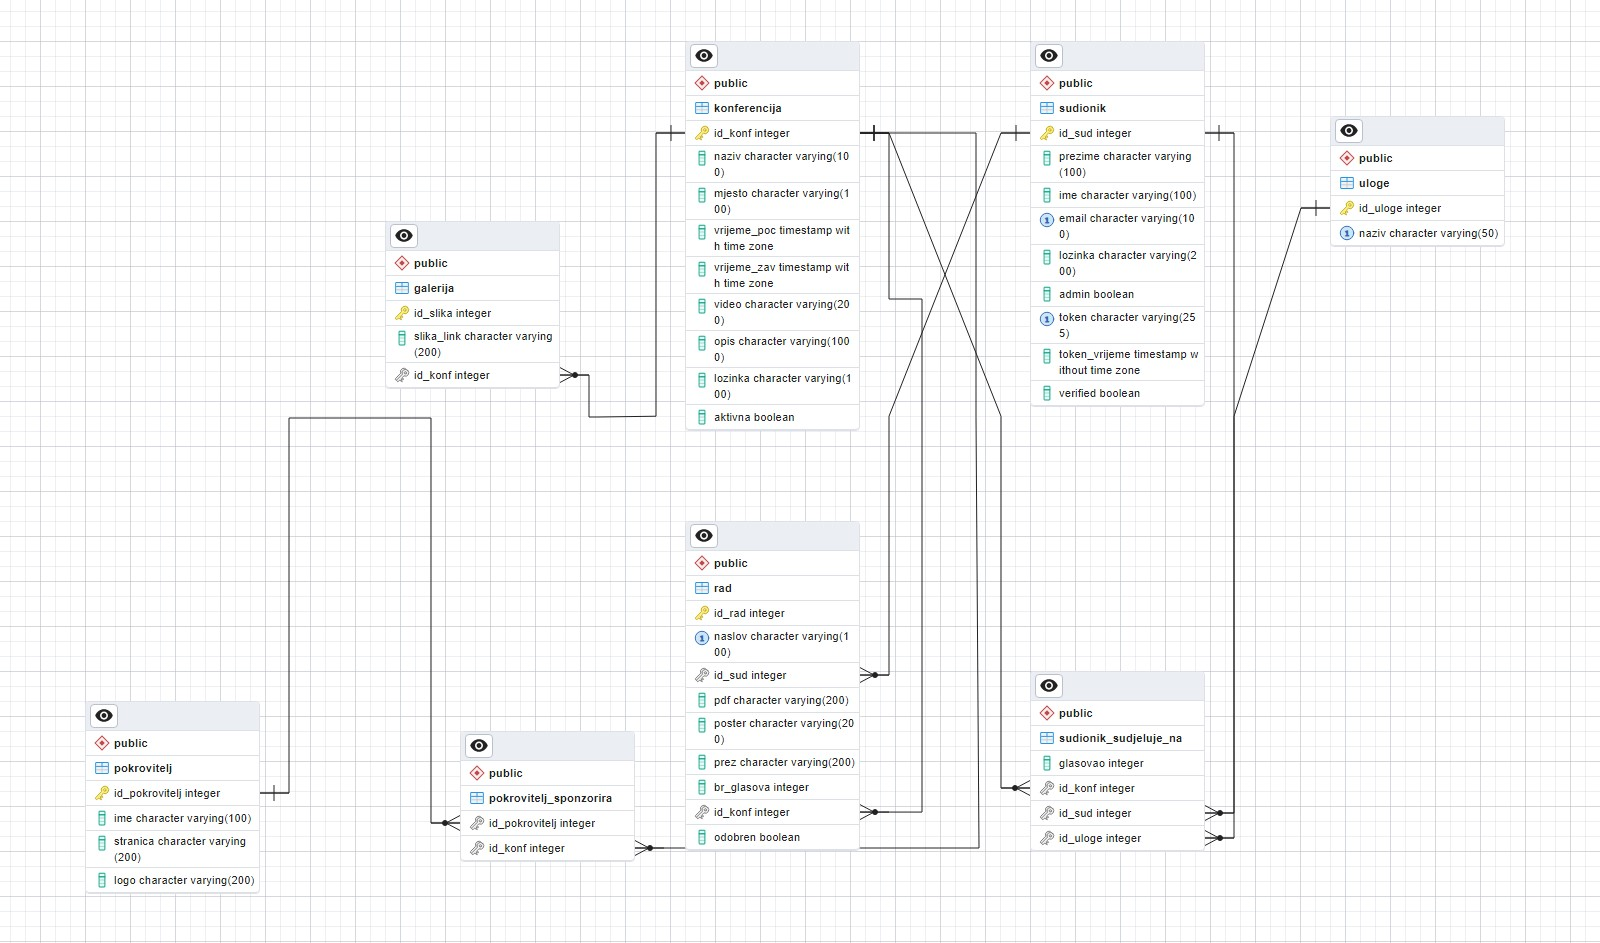
\includegraphics[width=15cm]{slike/dijagram.jpg}
	\caption{Slika 4.1: Dijagram baze podataka}
	\label{fig:fer-logo}
\end{figure}
			
			\eject
			
			
		\section{Dijagram razreda}
		
			\text{}Na slici ispod je prikazan raspored backend-a. Slika 4.2/a prikazuje uloge te funkcije kojima svaka od uloga može pristupiti. Te funkcije manipuliraju s podacima u bazi podataka dok su u modelima spremljeni atributi tablica baze podataka. Datoteka models preslikava strukturu baze podataka u aplikaciju. Funkcije koje su implementirane u datoteci routes, a iste su kao i funkcije prikazane kod voditelja, vraćaju JSON datoteke s html status kodom te dohvaćaju i spremaju podatke u bazu podataka.\\
			
			\text{}
			
			\begin{figure}
				\centering
				\begin{subcaption}[htb]
					
					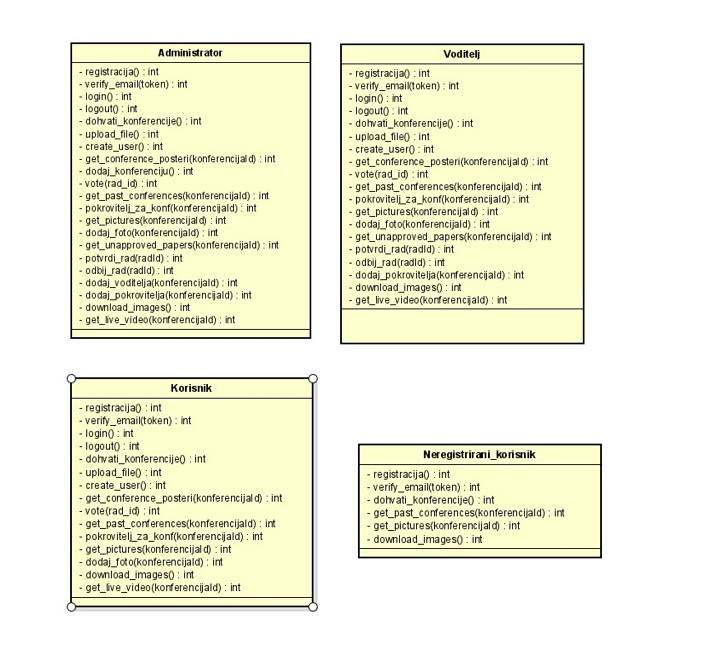
\includegraphics[width=12cm]{slike/zajednoooooooo.jpg}

					\label{fig:fer-logo}
				\end{subcaption}%
				\begin{subcaption}[htb]
					
					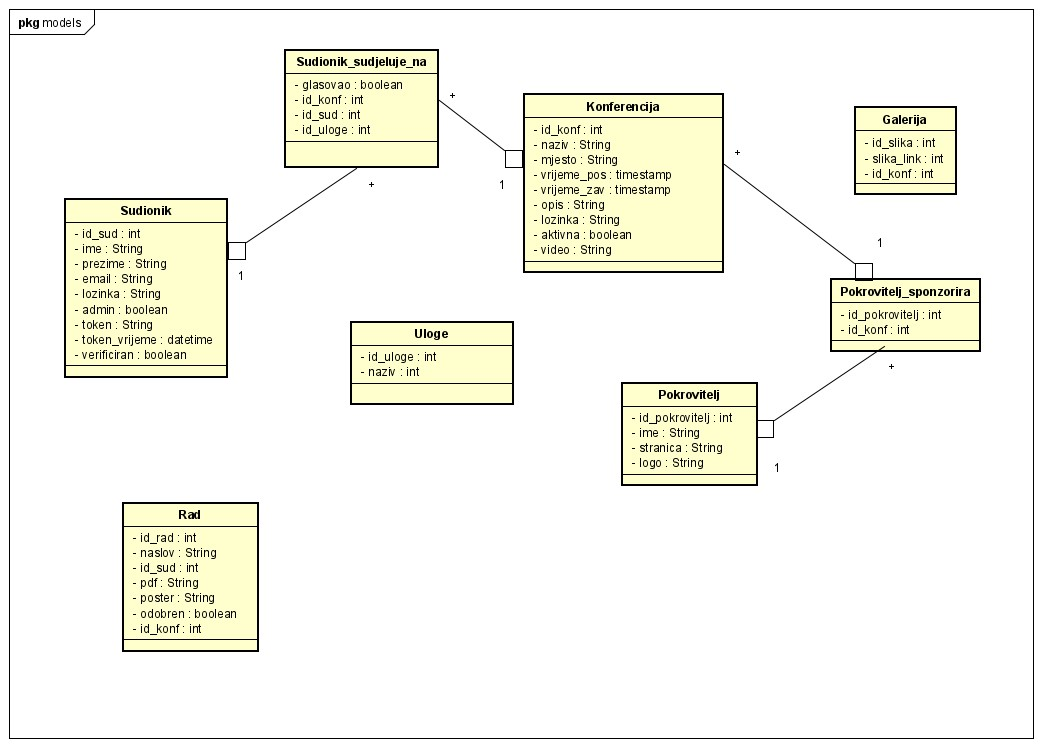
\includegraphics[width=12cm]{slike/models.jpg}

					\label{fig:fer-logo}
				\end{subcaption}
				
				\caption{Dijagram razreda - model baze podataka i uloge}
			\end{figure}
			
			
			
			\eject
		
		\section{Dijagram stanja}
			
			

			
			\textit{}Dijagram stanja prikazuje stanja objekta te prelaze iz stanja u stanje na određene akcije korisnika. Na slici ispod 4.3 prikazan je dijagram stanja za administratora. Nakon prijave administratoru se prikazuju sve trenutne i nadolazeće konferencije te u sve aktivne konferencije može pristupiti, dodati pokrovitelja, pregledati galeriju ili dodati fotografije u galeriju te pregledati radove i dati glas nekom radu po želji. U sve nadolazeće konferencije može dodati pokrovitelja, dodati rad, dodati voditelja te odobriti rad za prikazivanje na toj konferenciji. Također klikom na prošle konferencije može pregledati rezultate prošlih konferencija te preuzeti slike fotografirane na tim konferencijama.
			
			\begin{figure}[htb]
				\centering
				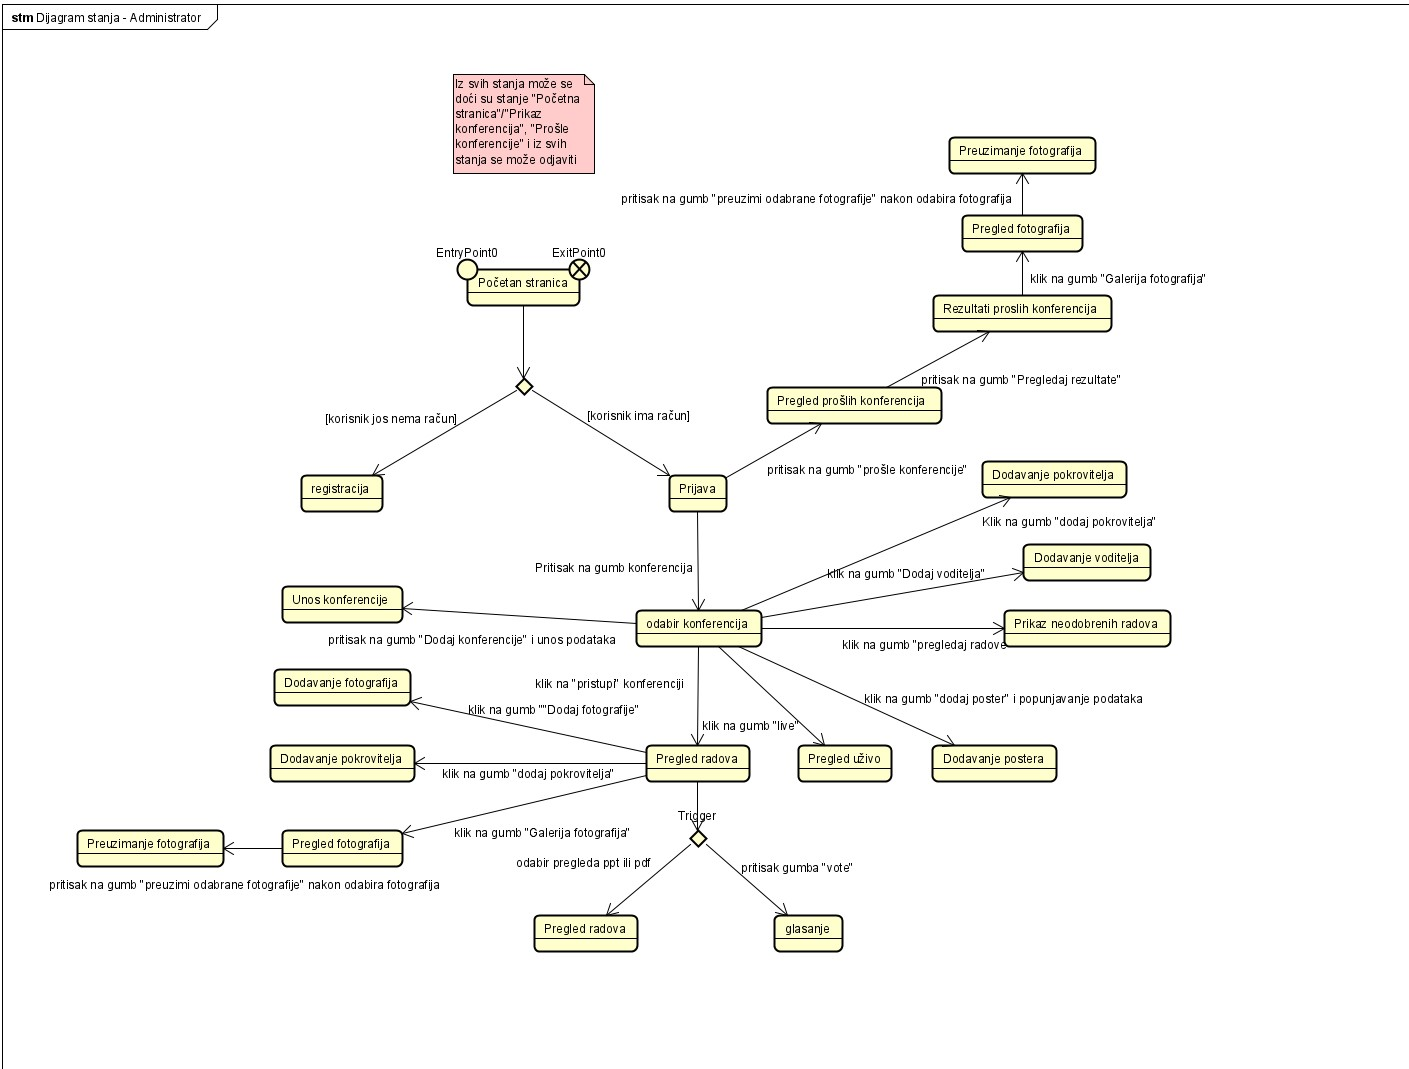
\includegraphics[width=15cm]{slike/Dijagram_stanja_admin.jpg}
				\caption{Dijagram stanja}
				\label{fig:fer-logo}
			\end{figure}
			
			\eject 
		
		\section{Dijagram aktivnosti}
			
			
			 \textit{}Dijagram aktivnosti primjenjuje se za opis modela toka upravljanja ili toka podataka. U priloženom dijagramu svako novi korak slijedi nakon završenog prethodnog koraka. Na slici 4.4 prikazan je proces glasanja. Korisnik se mora prijaviti u sustav, odabira konferenciju u kojoj želi pregledati radove te pristupa istoj ako zna lozinku za pristup. Nakon pristupa konferenciji pregledava radove i daje svoj glas jednom odabranom radu.
			 
			 \begin{figure}[htb]
			 	\centering
			 	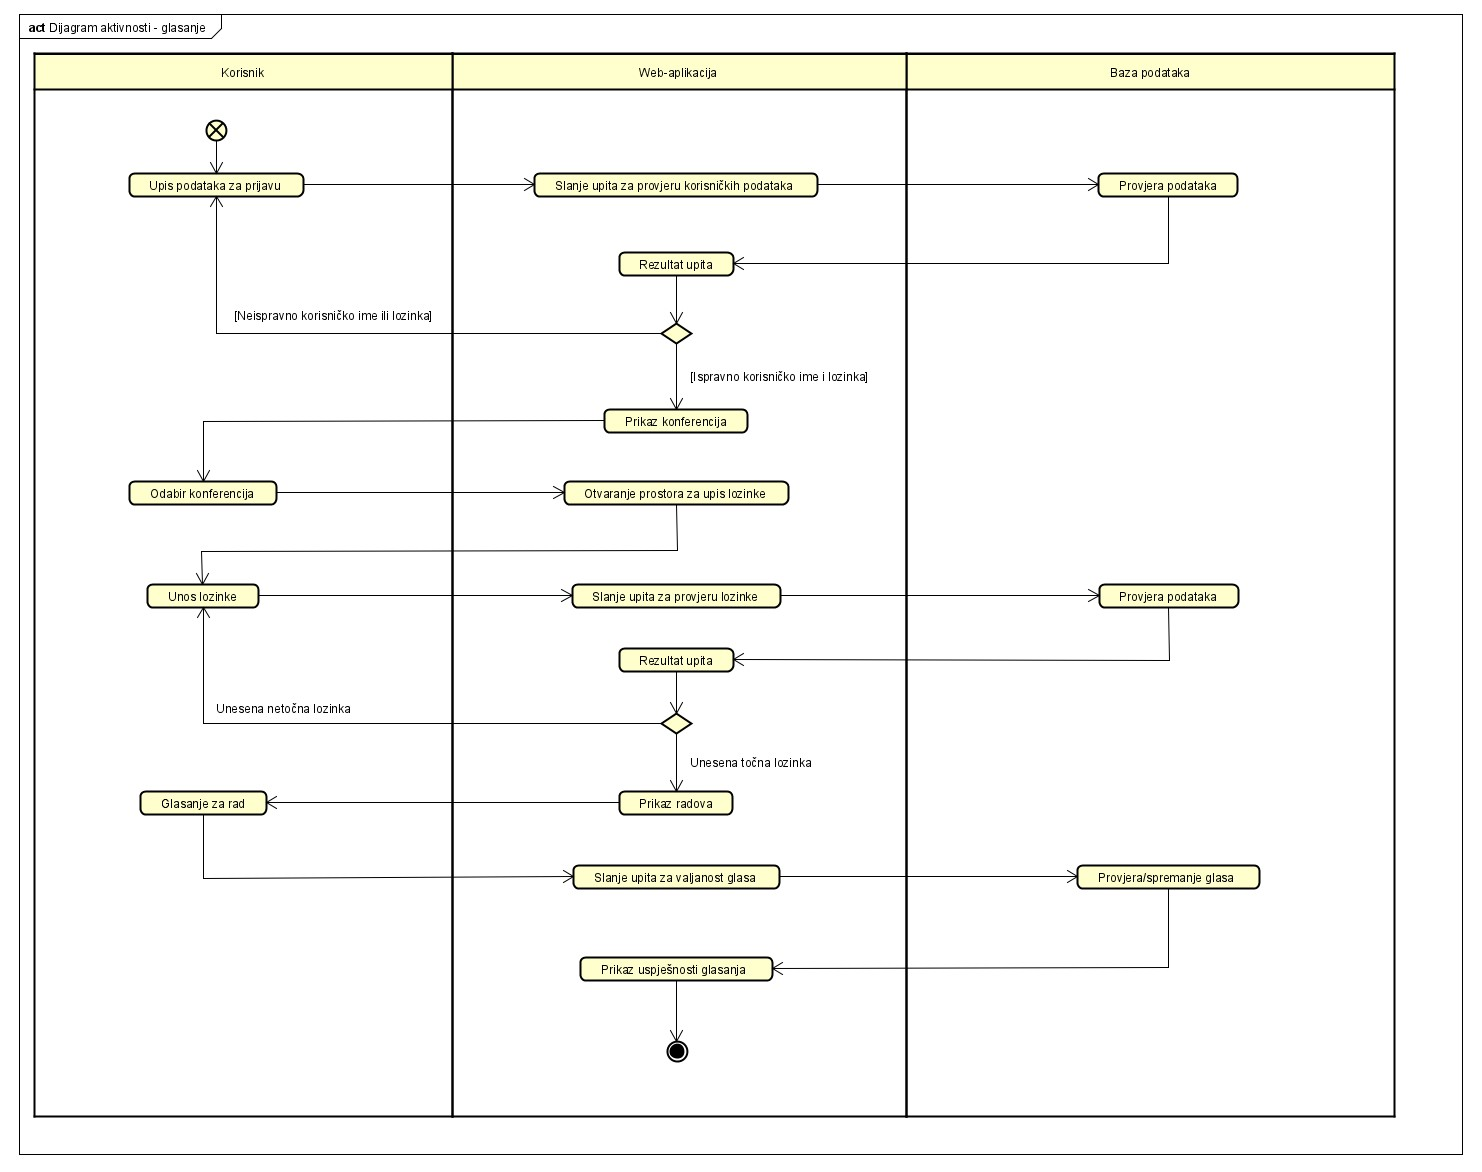
\includegraphics[width=15cm]{slike/Dija_aktivnosti_glasanja.jpg}
			 	\caption{Dijagram aktivnosti}
			 	\label{fig:fer-logo}
			 \end{figure}
			
			\eject
		\section{Dijagram komponenti}
		

		
			 \textit{}Dijagram komponenti prikazan na slici 4.5 opisuje organizaciju i međuovisnost komponenti, interne strukture i odnose prema okolini. Sustavu se pristupa preko dva različita sučelja. Preko sučelja za dohvat HTML, CSS i JS datoteka poslužuju se datoteke koje pripadaju frontend dijelu aplikacije. Router je komponenta koja na upit s url odgovara s nekom datotekom te se ovisno o ulozi na frontendu određuje što se prikazuje korisniku. Frontend se sastoji od niza JavaScript datoteka koje su raspoređene u cjeline po tipovima prikazanih frontend dokumenata. Sve JavaScript datoteke ovise o React biblioteci iz koje dohvaćaju gotove komponente. Preko sučelja flask pristupa se funkcijama za dohvat JSON podataka. Flask poslužuje podatke koji pripadaju backend dijelu aplikacije. SQLAlchemy je zadužen za dohvaćanje tablica iz baze podataka pomoću SQL upita.
			 
			  \begin{figure}[htb]
			 	\centering
			 	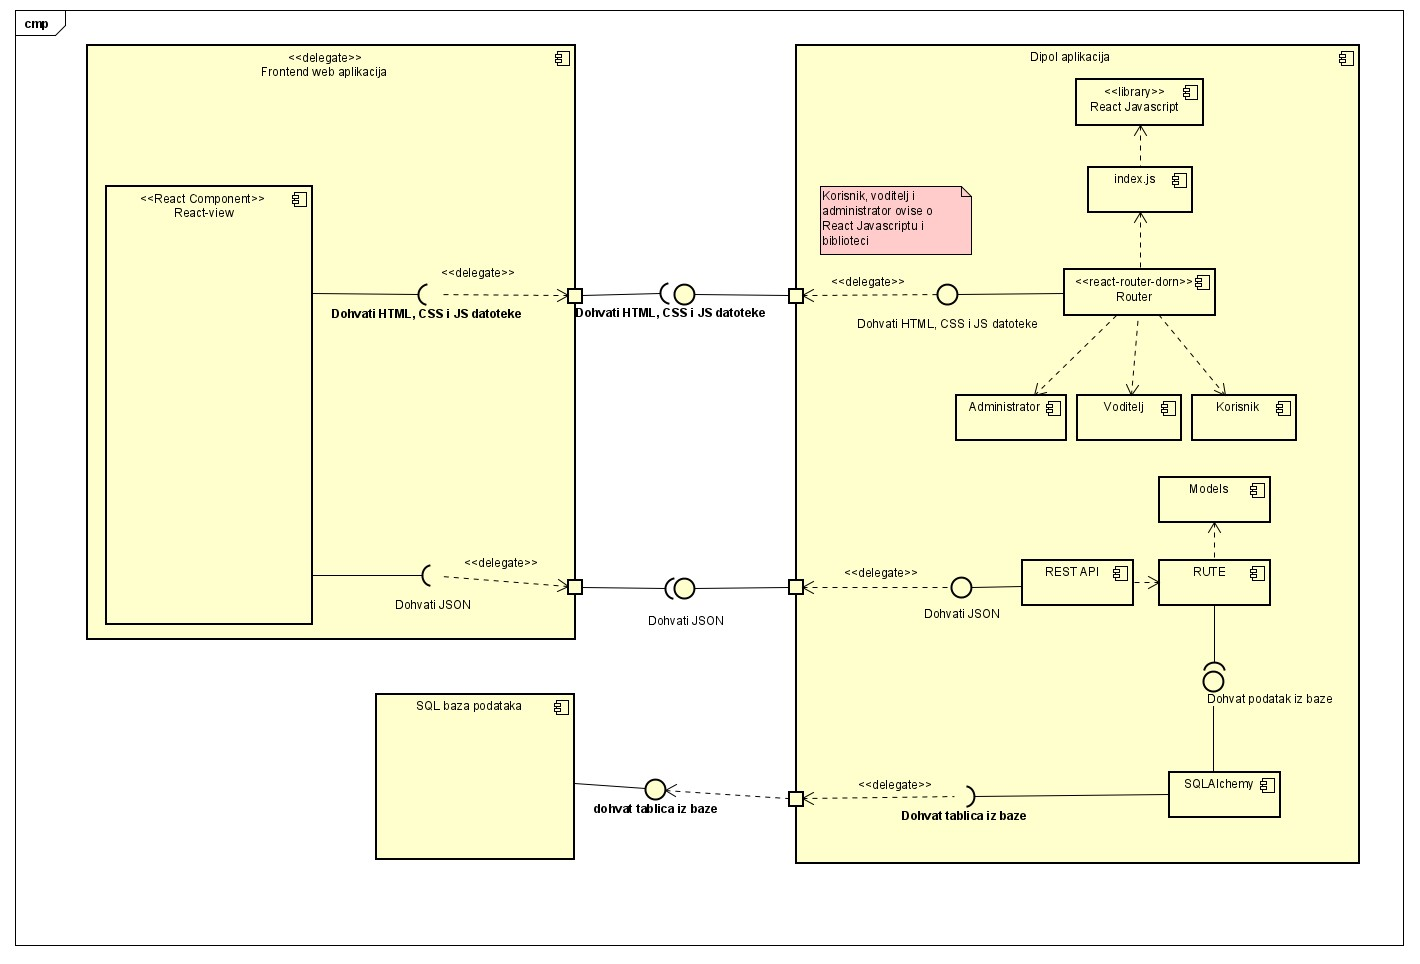
\includegraphics[width=15cm]{slike/Dijagram_komponensti.jpg}
			 	\caption{Dijagram komponenti}
			 	\label{fig:fer-logo}
			 \end{figure}